\documentclass[poisson.tex]{subfiles}
\begin{document}
\section{Navier Stokes com variáveis primitivas}
A equação de Navier Stokes é apresentada abaixo, essa é a equação que governa a dinâmica dos fluidos.

\begin{eqnarray}
\NavierStokesEq{\textbf{v}}{\textbf{f}}{navierstokes}\\
\NScondition{\textbf{v}}
\end{eqnarray}

\paragraph{} Neste trabalho consideraremos um campo vetorial de duas dimensões. A equação de Navier Stokes é altamente não-linear. Isso ocorre devido ao termo de convecção (aceleração independente do tempo, $\textbf{v}\cdot \nabla\textbf{v}$) e o termo da pressão $\nabla p$. 

\paragraph{} O método de Chorin com malha escalonada será utilizado. Para cada passo de tempo, há 3 etapas a serem realizadas. 
\paragraph{} Valores que devem ser fornecidas antes de se resolver tal equação são os parâmetros do fluido, $\mu$ e $\rho$ (massa específica), a força externa e as condições de fronteira. 
\subsection{Resolução Numérica}
\subsubsection{Time-splitting} A primeira etapa neste método de resolução é o \textit{time-splitting}. A discretização no tempo tem duas etapas. Para se entender isso, começamos com a equação abaixo:
\begin{equation}
\frac{\partial \textbf{v}}{\partial t}\approx \frac{\textbf{v}^{n+1}-\textbf{v}^n}{\Delta t}=\frac{\textbf{v}^{n+1}-\textbf{v}^*}{\Delta t}+\frac{\textbf{v}^{*}-\textbf{v}^n}{\Delta t} 
\end{equation}

A ideia do \textit{time-splitting} é responsabilizar cada um dos termos do lado direito desta equação com uma parte da equação de Navier-Stokes.

Reescrevendo a equação de Navier-Stokes:

\begin{eqnarray*}
\frac{\textbf{v}^{n+1}-\textbf{v}^*}{\Delta t}+\frac{\textbf{v}^{*}-\textbf{v}^n}{\Delta t}=-\frac{1}{\rho}\nabla p + \nu\nabla ^2 \textbf{v} + \frac{\textbf{f}}{\rho} - \textbf{v}\cdot \nabla \textbf{v}
\end{eqnarray*}

Agora, é possível impor o seguinte:

\begin{eqnarray}
\frac{\textbf{v}^{*}-\textbf{v}^n}{\Delta t}&=& \nu\nabla ^2 \textbf{v} + \frac{\textbf{f}}{\rho} - \textbf{v}\cdot \nabla \textbf{v}\label{equacaovestrela}\\
\frac{\textbf{v}^{n+1}-\textbf{v}^*}{\Delta t}&=&-\frac{1}{\rho}\nabla p\label{equacaoprepressao}
\end{eqnarray}

A equação \ref{equacaovestrela} pode ser discretizada e então obtemos $\textbf{v}^*$. A equação \ref{equacaoprepressao}, por sua vez, não pode ser diretamente discretizada e resolvida pois não se sabe $\textbf{v}^{n+1}$. No entanto, se o gradiente da equação for obtido, tem-se:

\begin{eqnarray*}
\nabla\cdot \left(\frac{\textbf{v}^{n+1}-\textbf{v}^*}{\Delta t}\right)&=&\nabla\cdot\frac{\textbf{v}^{n+1}}{\Delta t}-\nabla\cdot \frac{\textbf{v}^*}{\Delta t}\\
&=&-\frac{1}{\rho}\nabla^2 p
\end{eqnarray*}

A equação da continuidade $\nabla\cdot \textbf{v}=0$ tem de valer para $\textbf{v}^{n+1}$, logo:

\begin{eqnarray}
\nabla^2 p = \frac{\rho}{\Delta t}\nabla\cdot\textbf{v}^*\label{eqpressao}
\end{eqnarray}

Nos próximos passos, iremos (1) resolver para o tempo ``*'', que seria o intermediário entre $n$ e $n+1$, (2) obter a pressão (3) obter $n+1$.

\subsubsection{Desconsiderando a pressão}
\paragraph{} Numericamente, O primeiro passo é resolver a equação \ref{equacaovestrela}, que não leva em conta a pressão. Nas equações abaixo foi realizada a discretização da equação com essa simplificação. A parte direita de cada equação é avaliada no tempo passado, enquanto a parte da esquerda é avaliada para o próximo passo de tempo que deve ser obtido.

\begin{eqnarray}
\textbf{v}_{ij}^s&=&(\SumFour{u})\textbf{i} \nonumber \\&+& (\SumFour{v})\textbf{j}\\
\textbf{v}_{ij}^t&=&0.25(u_{ij}^n+u_{i+1j}^n+u_{i+1j-1}^n+u_{ij-1}^n)\textbf{i} \nonumber \\ &+& 0.25(v_{ij}^n+v_{i-1j}^n+v_{i-1j+1}^n+v_{ij+1}^n)\textbf{j}
\end{eqnarray}
%------------------- u* -------------------
\begin{eqnarray}
u_{ij}^{*}&=&u_{ij}^n+\frac{\Delta t}{\rho}\left[\mu\left(\frac{u_{ij}^s-4u_{ij}^n}{\Delta
x^2}\right)+Fx_{ij}^n\right] + \nonumber \\
&-&\left[u_{ij}^n(u_{i+1j}^n-u_{i-1j}^n)+v_{ij}^t(u_{ij+1}^n-u_{ij-1}^n)\right]\frac{\Delta t}{2\Delta x}
\end{eqnarray}
%------------------- v* ------------------
\begin{eqnarray}
v_{ij}^{*}&=&v_{ij}+\frac{\Delta t}{\rho}\left[\mu\left(\frac{v_{ij}^s-4v_{ij}^n}{\Delta
x^2}\right)+Fy_{ij}^n\right] \nonumber \\
&-&\left[u_{ij}^t (v_{i+1j}^n-v_{i-1j}^n)+v_{ij}^n(v_{ij+1}^n-v_{ij-1}^n)\right]\frac{\Delta t}{2\Delta x}
\end{eqnarray}

\paragraph{} Note que as equações acima são só válidas para pontos internos à malha escalonada. Os pontos de fronteira serão obtidos por equações diferentes. Considere a parede da esquerda da cavidade, onde a velocidade normal é 0. Como nossa malha é escalonada, este ponto não está salvo na matrix e uma média deve ser feita de modo a determinar o ponto da fronteira da malha. Neste caso, teria-se:

\begin{eqnarray*}
\frac{v_{i-\frac{1}{2}j}+v_{i+\frac{1}{2}j}}{2}=0
\end{eqnarray*}

o que leva a:
\begin{eqnarray}
v_{i-\frac{1}{2}j} &=& -v_{i+\frac{1}{2}j}
\end{eqnarray}

De maneira similar, para as paredes de baixo e da direita, tem-se:

\begin{eqnarray}
u_{ij-\frac{1}{2}}&=&-u_{ij+\frac{1}{2}}\\
v_{i+\frac{1}{2}j} &=& -v_{i-\frac{1}{2}j}
\end{eqnarray}

Para a parte de cima, onde a velocidade é diferente de zero, tem-se:

\begin{eqnarray*}
\frac{u_{ij+\frac{1}{2}}+u_{ij-\frac{1}{2}}}{2}=u_{Bi}
\end{eqnarray*}

$u_{Bi}$ é a condição de fronteira para o ponto na coluna $i$.


Retirando os índices fracionários:

\begin{eqnarray}
v_{i-1j} &=& -v_{ij},\,\, \textrm{esquerda}\\
u_{ij-1}&=&-u_{ij},\,\, \textrm{embaixo} \\
v_{ij} &=& -v_{i-1j},\,\, \textrm{direita}\\
u_{ij} &=& 2u_{Bi}-u_{ij-1},\,\, \textrm{em cima}
\end{eqnarray}

fixando o índice de cada lado:

\begin{eqnarray}
v_{0j} &=& -v_{1j},\,\, \textrm{esquerda}\\
u_{i0}&=&-u_{i1},\,\, \textrm{embaixo} \\
v_{n-1j} &=& -v_{n-2j},\,\, \textrm{direita}\\
u_{in-1} &=& 2u_{Bi}-u_{in-2},\,\, \textrm{em cima}
\end{eqnarray}



\paragraph{} Com isto, tem-se \[\textbf{v}^{*}=(u^*,v^*)\]
%------------------------Obter a pressão!!!! --------------------
\subsubsection{Obter a pressão}
\paragraph{} Tirando o divergente das equações vetoriais, tem-se a seguinte equação:
\begin{equation}
\nabla^2 p = \frac{\rho}{\Delta t} \nabla\cdot \textbf{v}^*=\frac{\rho}{\Delta t} 
\left( \frac{\partial u^*}{\partial x}+\frac{\partial v^*}{\partial y} \right)
\end{equation}
\paragraph{} Dado ter-se um sistema resolvendo a equação de poisson, basta-se calcular o termo da direita e colocar como não-homogeneidade.
\begin{equation}
DIV_{ij}=\frac{\rho}{\Delta t}\left( \frac{u_{i+1j}^*-u_{ij}^*}{\Delta x}+\frac{v_{ij+1}^*-v_{ij}^*}{\Delta x}\right)
\end{equation}
\paragraph{} As condições de contorno são todas de Neumann. Para pontos internos à malha, tem-se:
\begin{equation}
p_{ij}=\frac{1}{4}[(p_{i+1j}+p_{i-1j}+p_{ij+1}+p_{ij-1})-\Delta x^2 DIV_{ij}]
\end{equation}
\paragraph{} Quais pontos são internos à malha? São os pontos $x_{ij}$ em $D$ que é definido da seguinte maneira:
\begin{equation}
D = \{x_{ij}\,|\, 0\le i < N \textrm{ e } 0\le j < N \}
\end{equation}
\paragraph{} A rotina para Poisson com Neumann já está implementada. Falta agora
as condições de contorno nas fronteiras. Como obtê-las?
\paragraph{} Primeiramente, considere-se novamente a equação de Navier Stokes:
\[\rho\left( \frac{\partial \textbf{v}}{\partial t}+\textbf{v}\cdot\nabla\textbf{v}\right)=-\nabla p+\mu\nabla^2\textbf{v}+\textbf{f}\]
\[\nabla\cdot\textbf{v}=0\]
\paragraph{} Destrinchando a equação para duas coordenadas, tem-se:
\begin{eqnarray}
\frac{\partial u}{\partial t}+u\frac{\partial u}{\partial x}+v\frac{\partial
u}{\partial y}=-\frac{1}{\rho}\frac{\partial p}{\partial
x}+\nu\left(\frac{\partial^2 u}{\partial^2 x}+\frac{\partial^2 u}{\partial^2
y}\right)+f_x\\
\frac{\partial v}{\partial t}+u\frac{\partial v}{\partial x}+v\frac{\partial
v}{\partial y}=-\frac{1}{\rho}\frac{\partial p}{\partial
y}+\nu\left(\frac{\partial^2 v}{\partial^2 x}+\frac{\partial^2 v}{\partial^2
y}\right)+f_y
\end{eqnarray}
\paragraph{} Se fizermos uma análise dos pontos na parede da esquerda ou
direita, e aplicarmos as condições de impenetrabilidade e não-deslizamento, que
dizem que $u=0$ e $v=0$ na parede, temos a simplificação da equação, pois vários
termos se tornam zero. As equações para as duas paredes verticais é a seguinte:
\begin{equation}
\frac{\partial p}{\partial x}\Bigg|_{\textrm{parede}}=\rho\nu\frac{\partial^2
u}{\partial x^2}\Bigg|_{\textrm{parede}}+\rho f_x
\end{equation}
\paragraph{} Para as paredes que ficam na horizontal tem-se:
\begin{equation}
\frac{\partial p}{\partial y}\Bigg|_{\textrm{parede}}=\rho\nu\frac{\partial^2
v}{\partial y^2}\Bigg|_{\textrm{parede}}+\rho f_y
\end{equation}
\paragraph{Equações discretizadas para fronteira de Poisson} As equações, em
sequência, para as fronteiras da esquerda, direita, baixo e topo da matriz são
as seguintes:
\begin{eqnarray}
\frac{p_{0j}-p_{-1j}}{\Delta x}=\frac{\mu}{\Delta x^2}(2u_{ij}-5u_{i+1j}+4u_{i+2j}-u_{i+3j})+\frac{\rho}{2}(f_{ij}+f_{i+1j}) \label{pressure_01}\\
\frac{p_{nj}-p_{n-1j}}{\Delta x}=\frac{\mu}{\Delta x^2}(2u_{ij}-5u_{i-1j}+4u_{i-2j}-u_{i-3j})+\frac{\rho}{2}(f_{ij}+f_{i-1j})\label{pressure_02}\\
\frac{p_{i0}-p_{i-1}}{\Delta y}=\frac{\mu}{\Delta y^2}(2v_{ij}-5v_{ij+1}+4v_{ij+2}-v_{ij+3})+\frac{\rho}{2}(f_{ij}+f_{ij-1}) \label{pressure_03}\\
\frac{p_{in}-p_{in-1}}{\Delta y}=\frac{\mu}{\Delta y^2}(2v_{ij}-5v_{ij-1}+4v_{ij-2}-v_{ij-3})+\frac{\rho}{2}(f_{ij}+f_{ij-1}) \label{pressure_04}
\end{eqnarray}
\paragraph{} Agora, tem-se as equações que serão utilizadas no domínio em questão, na malha escalonada, para resolver a equação da pressão em Navier Stokes. Abaixo tem-se o nosso domínio.
\domainOne

\paragraph{} Cada um dos pontos pretos são pontos internos, e nestes pontos precisamos saber os valores das derivadas, de forma a obter a matriz $DIV$, para então utilizar na resolução da equação de Navier, que estamos originalmente interessados. Com a malha extendida, com a fronteira imaginária adicionada, ela fica no ``ponto'' para obter o gradiente de pressão usando derivadas centrais em cada um dos pontos, agora internos, da nossa malha extendida. As setas verticais indicam as velocidades horizontais, enquanto as setas verticais indicas velocidades verticais. 

\paragraph{} O modelo de cada bloco é o seguinte:

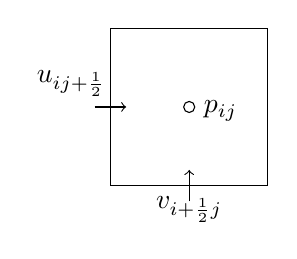
\begin{tikzpicture}
\draw (0,0) rectangle (2,2);
\draw (1.4,0.95) node {$p_{ij}$};
\draw[->] (1,-0.2) -- (1,0.2);
\draw (1,-0.3) node {$v_{i+\frac{1}{2}j}$};
\draw[->] (-0.2,1) -- (0.2,1);
\draw (-0.5,1.3) node {$u_{ij+\frac{1}{2}}$};
\draw (1,1) circle (2pt);
\end{tikzpicture}

\paragraph{} Para a representação no computador, somente com índices positivos, tem-se de mudar o local da origem, e fica-se com o seguinte esquema:
\esquemaUm

\paragraph{} As coordenadas dos pontos acima, onde os pontos são $x_{ij}$, são diferentes do original mencionado antes com uma malha escalonada com índices negativos, e as equações ficam com os termos de uma forma um pouco diferente. Em relação ao tamanho da matriz, note que para uma malha de ordem 6 como acima, a malha escalonada ficou de ordem 8. Logo, há um aumento da ordem da matriz por uma adição de 2 ordens.

\paragraph{} Reescrevendo as equação de \ref{pressure_01} até \ref{pressure_04}, e considerando $n$ a ordem da matriz, temos:
\begin{eqnarray}
i=1 \,|\, p_{i-1j}=p_{ij}-\frac{\mu}{\Delta x}\left(2u_{ij}-5u_{i+1j}+4u_{i+2j}-u_{i+3j}\right)-\frac{\rho\Delta x}{2}(f_{ij}+f_{i+1j})\\
i=n \,|\, p_{i+1j}=p_{ij}+\frac{\mu}{\Delta x}\left(2u_{ij}-5u_{i-1j}+4u_{i-2j}-u_{i-3j}\right)+\frac{\rho\Delta x}{2}(f_{ij}+f_{i+1j})\\
j=1 \,|\, p_{ij-1}=p_{ij}-\frac{\mu}{\Delta x}\left(2v_{ij}-5v_{ij+1}+4u_{ij+2}-u_{ij+3}\right)-\frac{\rho\Delta x}{2}(f_{ij}+f_{i+1j})\\
j=n \,|\, p_{ij+1}=p_{ij}+\frac{\mu}{\Delta x}\left(2v_{ij}-5v_{ij-1}+4u_{ij-2}-u_{ij-3}\right)+\frac{\rho\Delta x}{2}(f_{ij}+f_{i+1j})
\end{eqnarray}
\subsubsection{Resolver para o passo $t+\Delta t$}
\paragraph{} Finalmente, tem-se: 

\begin{equation}
\frac{\textbf{v}^{n+1}-\textbf{v}^*}{\Delta t}=-\frac{1}{\rho}\nabla p
\end{equation}
\paragraph{} Expandindo para as equações escalares, tem-se:
\begin{eqnarray}
u^{n+1}=u^*-\frac{\Delta t}{\rho}\frac{\partial p}{\partial x}\\
v^{n+1}=v^*-\frac{\Delta t}{\rho}\frac{\partial p}{\partial y}
\end{eqnarray}
\paragraph{} Basta discretizar os termos das derivadas parciais agora:

\begin{eqnarray}
p_{x,ij}=\frac{p_{ij}-p_{i-1j}}{\Delta x}\\
p_{y,ij}=\frac{p_{ij}-p_{ij-1}}{\Delta x}
\end{eqnarray}

\paragraph{} E finalmente tem-se a solução para o tempo $n+1$ a partir do tempo passado $n$:

\begin{eqnarray}
\NextTimeStep{u}{x}\\
\NextTimeStep{v}{y}
\end{eqnarray}
\paragraph{} Cada uma das varíaveis acima é uma matriz.
\end{document}
